\documentclass[final]{beamer}

\usetheme[subsectionpage=progressbar]{metropolis}
\setbeamertemplate{footline}{}


\usepackage[ruled]{algorithm2e}
\usepackage{animate}
\usepackage[backend=bibtex, style=numeric]{biblatex}
    \addbibresource{references}
\usepackage[font=footnotesize,labelformat=empty]{caption}
\usepackage{graphicx}
\usepackage{hyperref}
\usepackage{tikz}
    \usetikzlibrary{%
        arrows.meta,
        decorations.pathreplacing,
        decorations.text,
        patterns,
        shapes.arrows,
        shapes.geometric
    }


% TikZ styles, commands and settings
\definecolor{magenta}{RGB}{226, 62, 138}
\tikzstyle{every picture} += [remember picture]
\tikzstyle{na} = [baseline=-.5ex]

\tikzset{%
    column/.pic={%
        code{%
            \draw[line width=1pt] (0, 0) rectangle (-2cm, 4cm);
            \foreach \val in {0, ..., #1}{%
                \draw[rotate=90] ([xshift=-\val*10pt] 4cm, 2cm) -- ++(0, -2cm);
            };
            \node at (-1cm, 1.25) {$\vdots$};
            \foreach \val in {1, 2}{%
                \draw (0, \val * 10pt) -- ++(-2cm, 0);
            };
        }
    }
}

\tikzset{%
    fullcolumn/.pic={%
        code{%
            \draw[line width=1pt] (0, 0) rectangle (-2cm, #1*10pt);
            \foreach \val in {0, ..., #1}{%
                \draw[rotate=90] ([xshift=-\val*10pt] #1*10pt, 2cm) -- ++(0, -2cm);
            };
        }
    }
}


\title{%
    Evolutionary dataset optimisation:
    learning algorithm quality through evolution
}
\author{\large{Henry Wilde, Dr.\ Jonathan Gillard, Dr.\ Vincent Knight}}
\institute{%
    \vfill%
    \centering%
    
\includegraphics[height=.2\paperheight]{img/cu_logo.png}%
    \hspace{5pt}%
    
\includegraphics[height=.2\paperheight]{img/cthb_logo.jpg}
}
\date{}

\begin{document}

\frame{%
    \maketitle%
}

\section{Premise and motivation}

\frame{%
    \centering
    
\includegraphics[width=.5\textwidth]{img/hammer.png}
}

\frame{%
    \centering
    \begin{figure}
        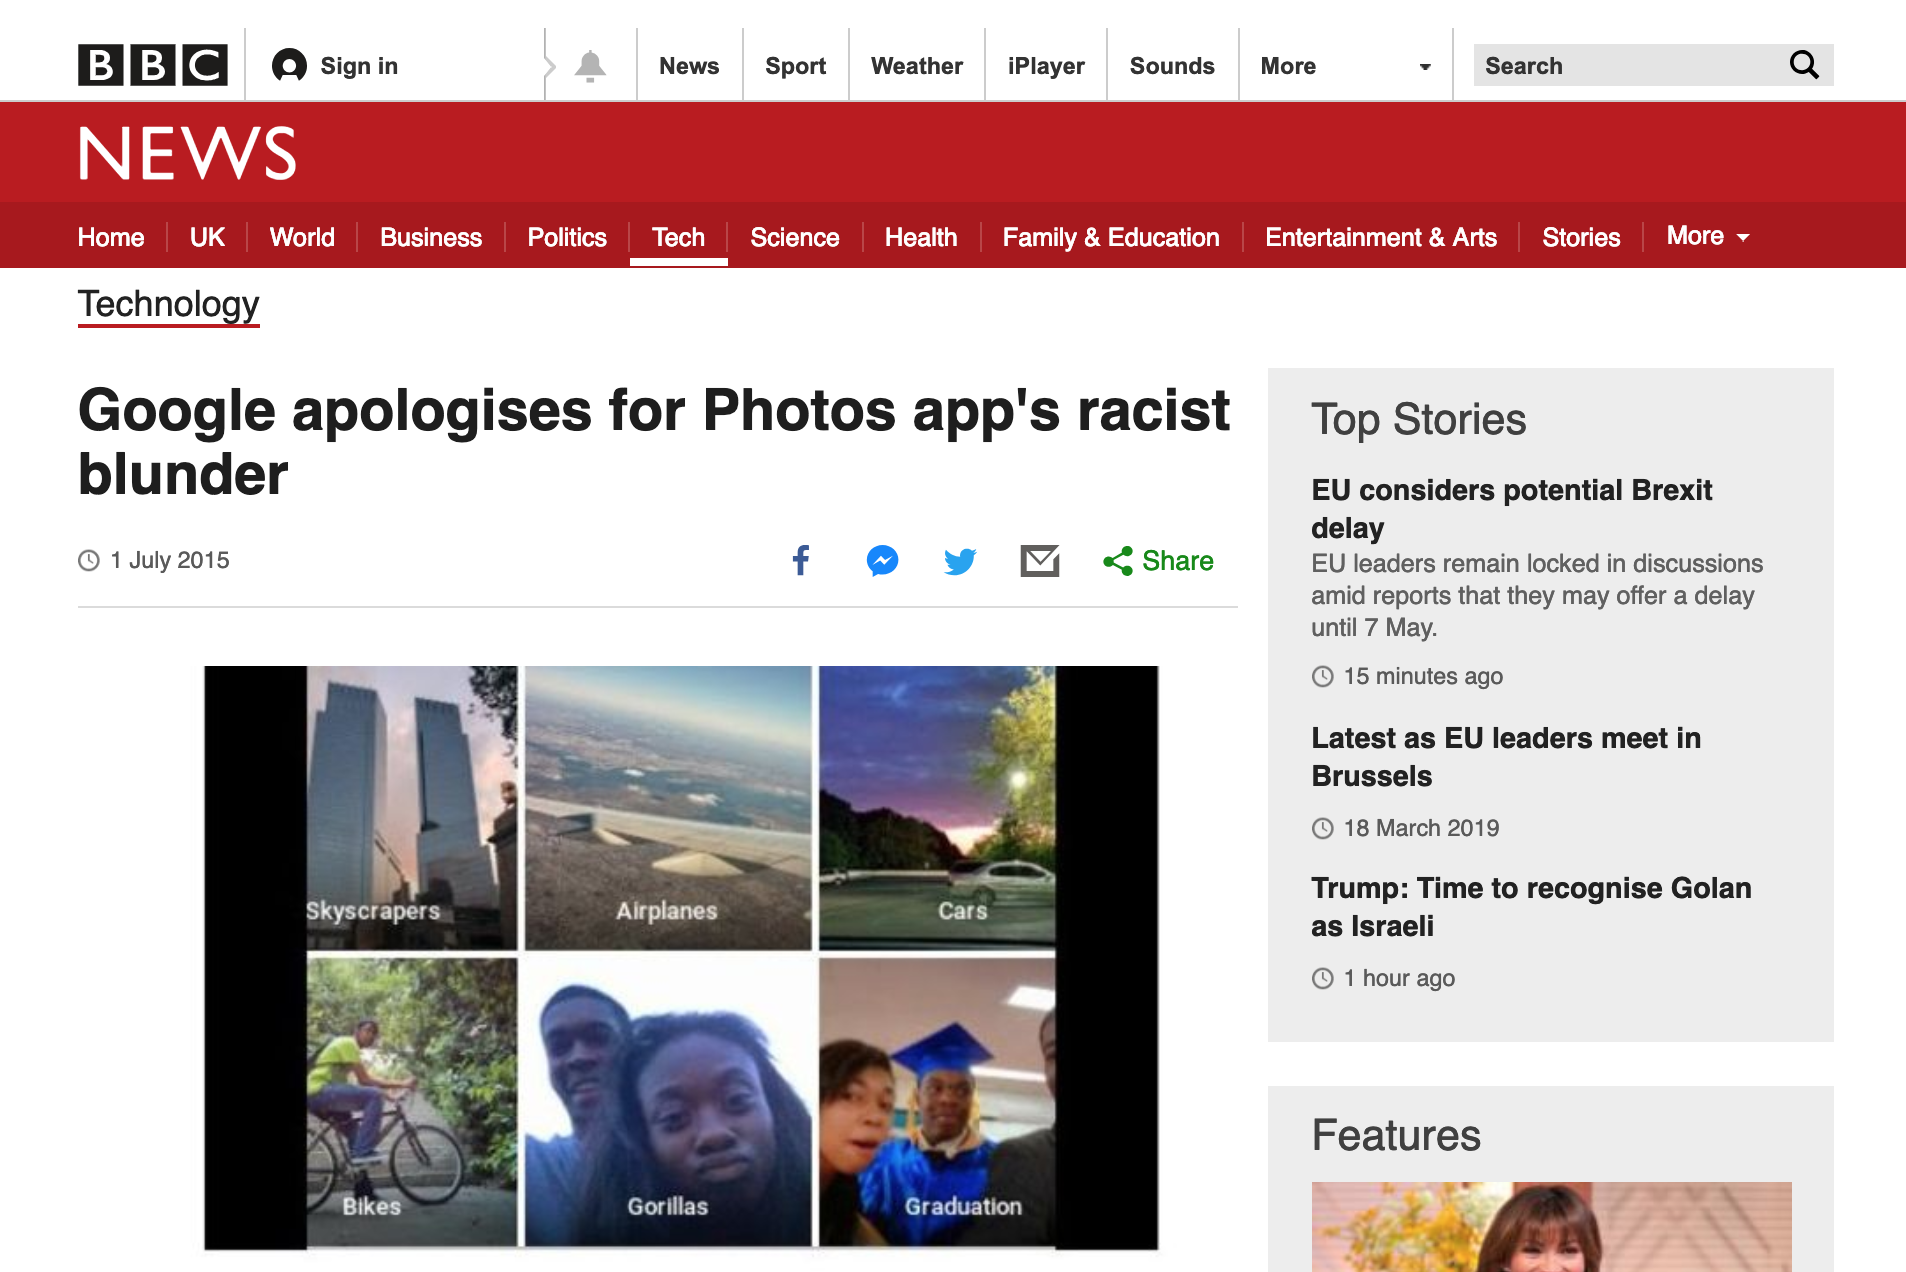
\includegraphics[width=.8\textwidth]{img/gorilla.png}
        \caption{%
            via: BBC News (\url{%
                https://www.bbc.co.uk/news/technology-33347866
            })
        }
    \end{figure}
}

\frame{%
    \begin{itemize}
        \item Hyndman reference (reliability)
        \item \fullcite{Torralba2011} (frailty)
    \end{itemize}
}

\frame{%
    Paradigm flip diagram
}

\subsection{Generating artificial data}

\frame{%
    \centering
    \begin{figure}
        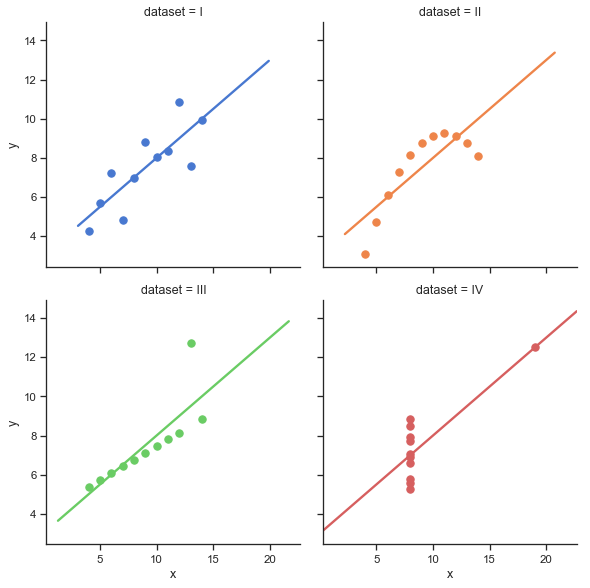
\includegraphics[width=.5\textwidth]{img/anscombes.png}
        \caption{%
            via: \url{%
                https://seaborn.pydata.org/examples/anscombes_quartet.html
            }
        }
    \end{figure}
}

\frame{%
    \centering
    \begin{figure}
        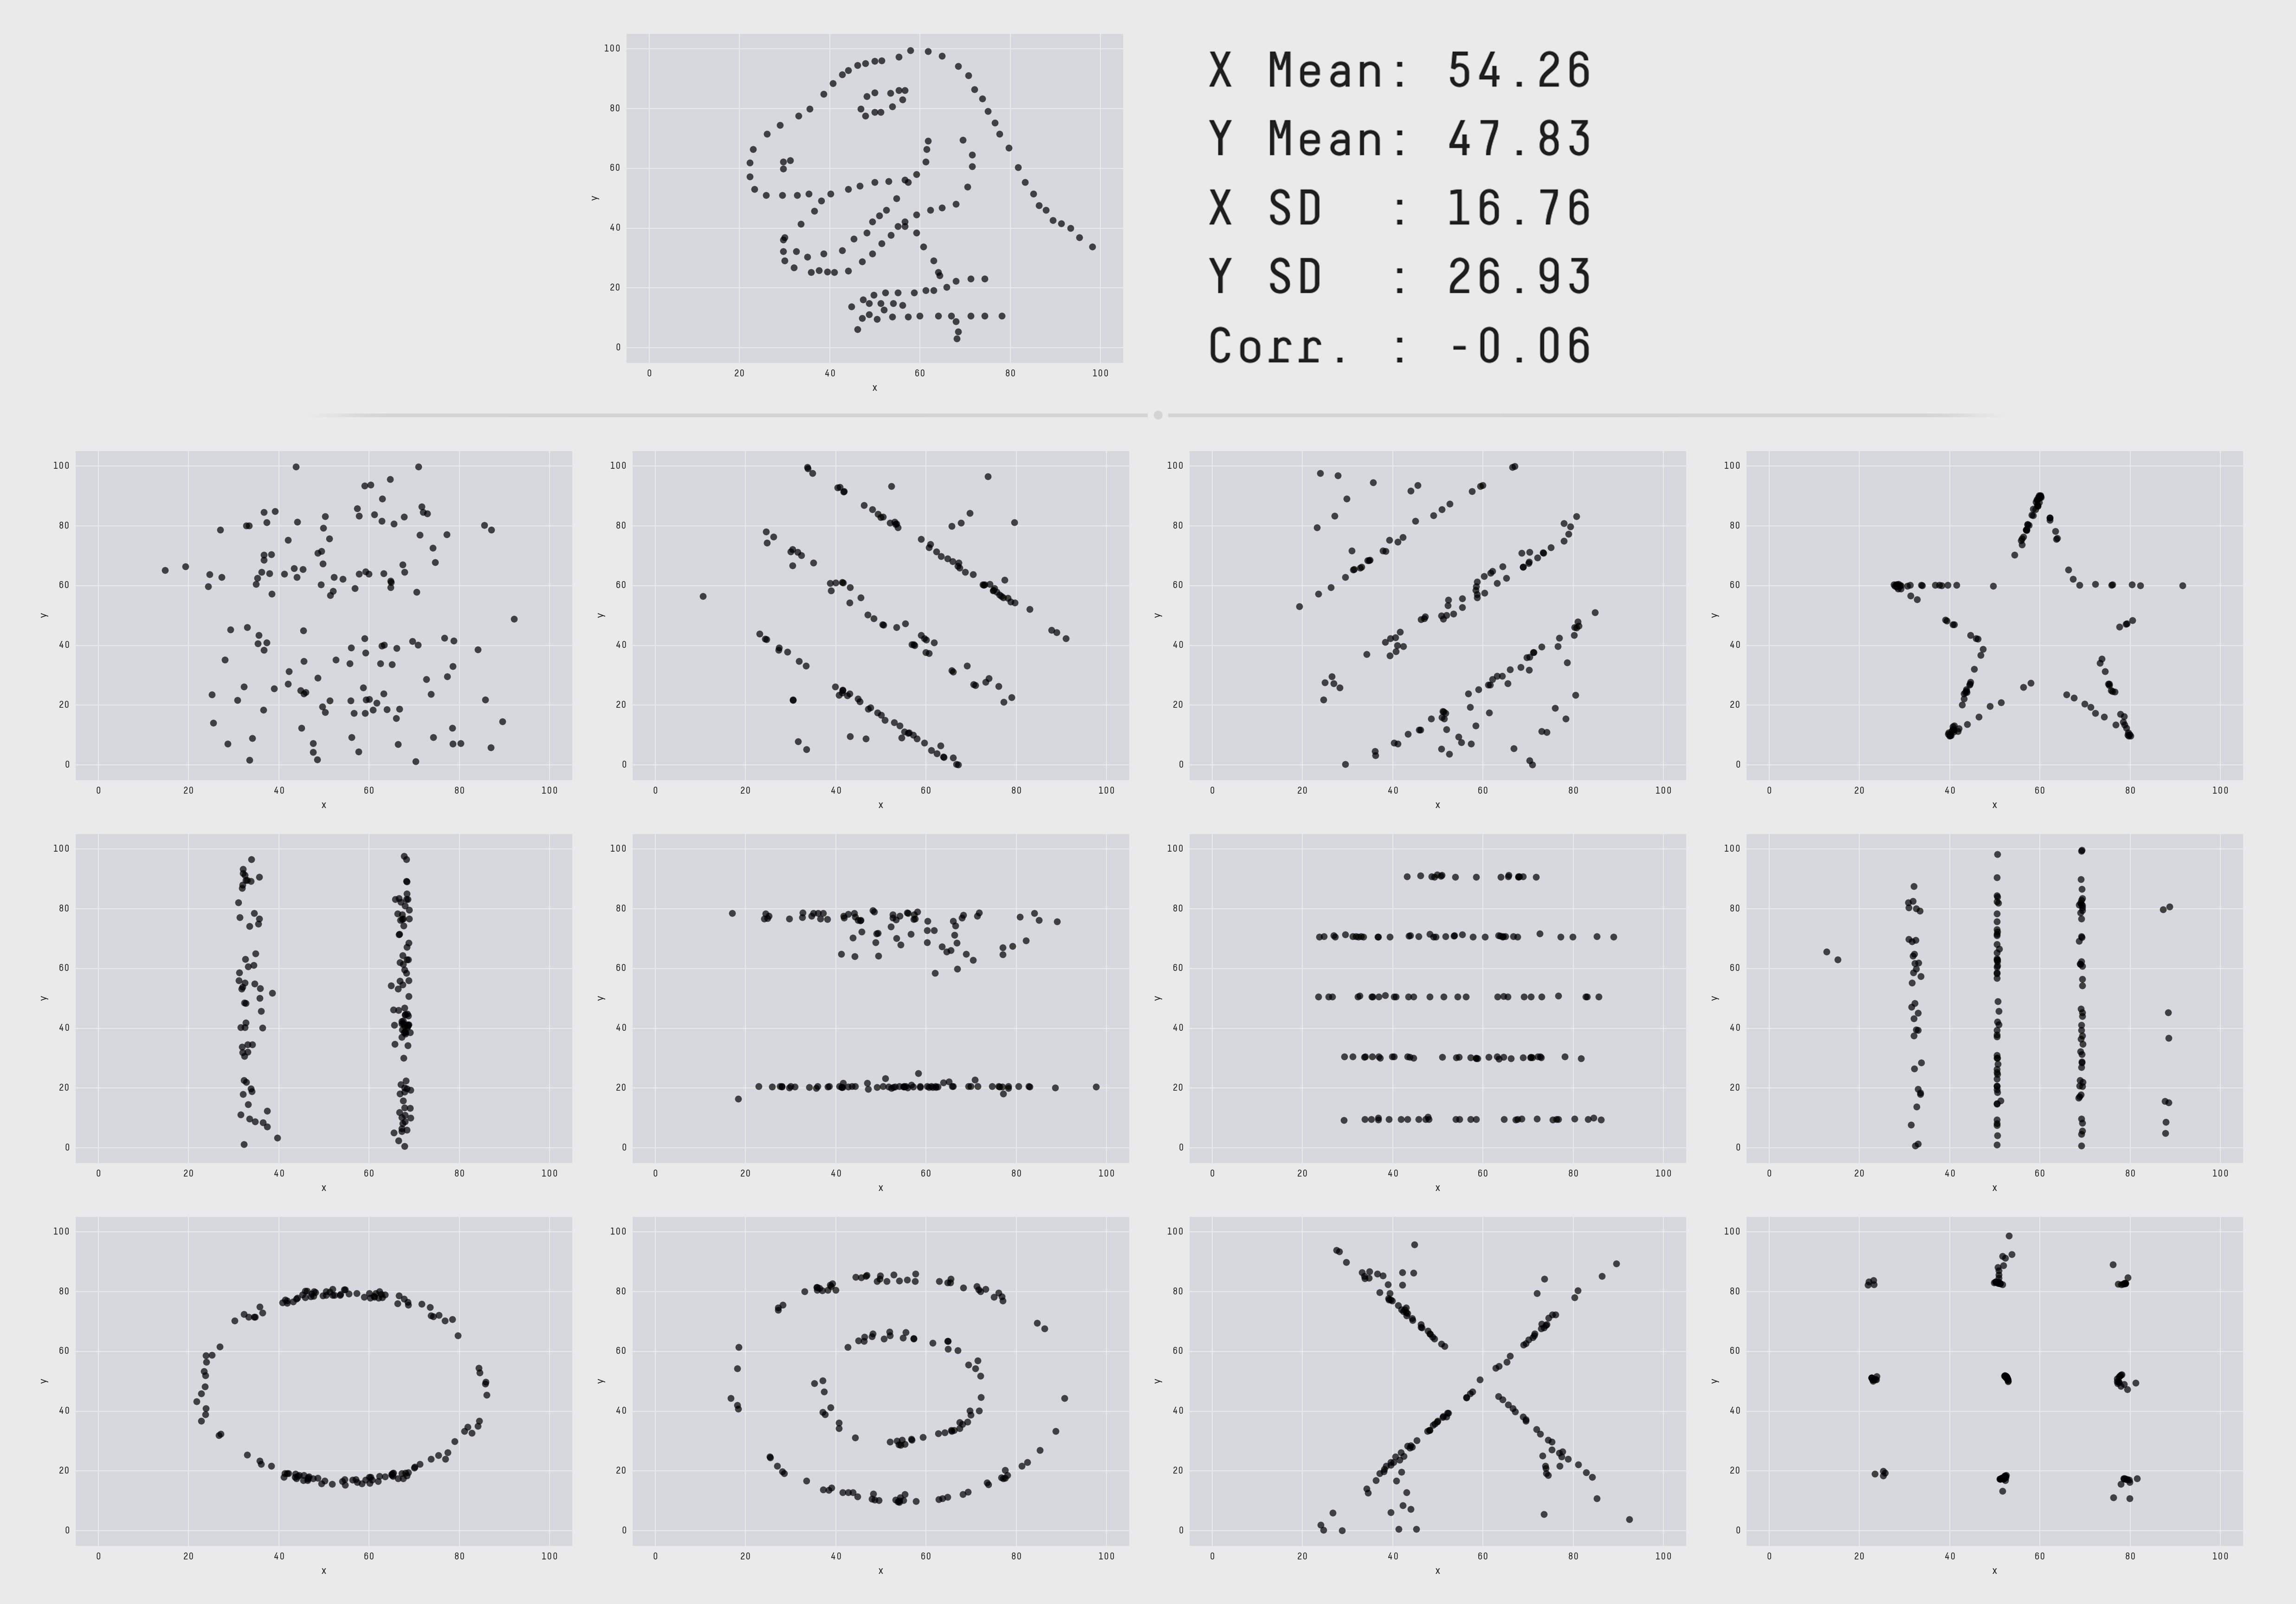
\includegraphics[width=.8\textwidth]{img/dino.png}
        \caption{%
            via: \url{%
                https://www.autodeskresearch.com/publications/samestats
            }
        }
    \end{figure}
}

\frame{%
    Dataset similarity diagram
}

\frame{%
    \huge{%
        Given some algorithm, how can one find data for which it performs well?
    }
}

\section{What is an evolutionary algorithm?}

\frame{%
    \resizebox{\textwidth}{!}{%
        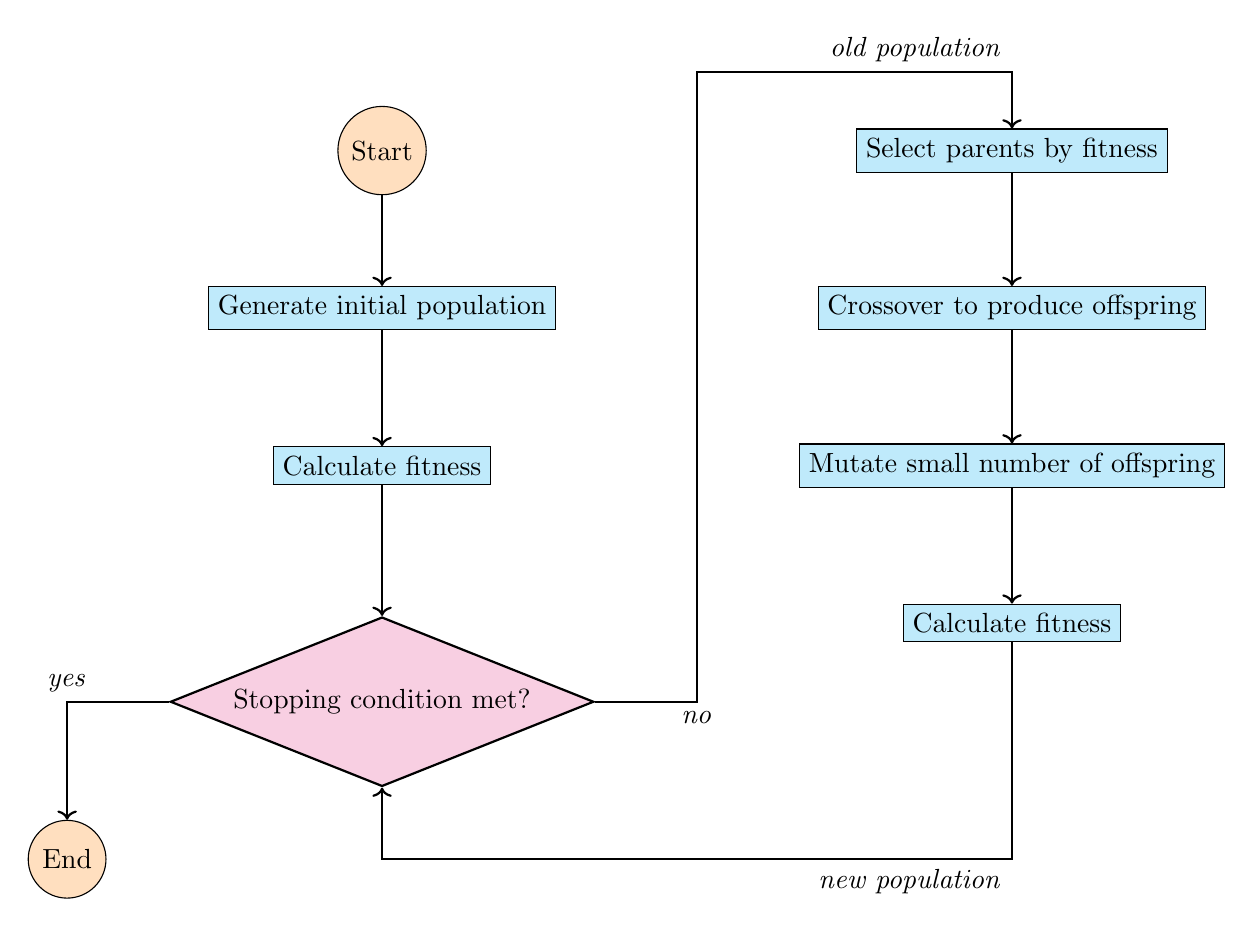
\begin{tikzpicture}
	\node[draw, circle, fill=orange!25] (start) at (0, 0) {Start};
    \node[draw, fill=cyan!25] (initial) at (0, -2) {Generate initial
        population};
    \node[draw, fill=cyan!25] (init-fitness) at (0, -4) {Calculate fitness};
    \node[draw, diamond, thick, aspect=2.5, fill=magenta!25] (stop) at (0, -7)
        {Stopping condition met?};
    \node[draw, circle, fill=orange!25] (end) at (-4, -9) {End};
    \node[draw, fill=cyan!25] (selection) at (8, 0) {Select parents by fitness};
    \node[draw, fill=cyan!25] (crossover) at (8, -2) {Crossover to produce
        offspring};
    \node[draw, fill=cyan!25] (mutation) at (8, -4) {Mutate small number of
        offspring};
    \node[draw, fill=cyan!25] (new-fitness) at (8, -6) {Calculate fitness};

    \draw[->, thick] (start) -- (initial);
    \draw[->, thick] (initial) -- (init-fitness);
    \draw[->, thick] (init-fitness) -- (stop);
    \draw[->, thick] (stop) -- (-4, -7) node[above] {\textit{yes}} -- (end);
    \draw[->, thick] (stop) -- (4, -7) node[below] {\textit{no}} -- (4, 1)
        -- (8, 1) node[above left] {\textit{old population}} -- (selection);
    \draw[->, thick] (selection) to (crossover);
    \draw[->, thick] (crossover) to (mutation);
    \draw[->, thick] (mutation) to (new-fitness);
    \draw[->, thick] (new-fitness) -- (8, -9) node[below left] {\textit{new
        population}} -- (0, -9) -- (stop);
\end{tikzpicture}

    }
}

\frame{%
    GA example
}

\frame{%
    \resizebox{\textwidth}{!}{%
        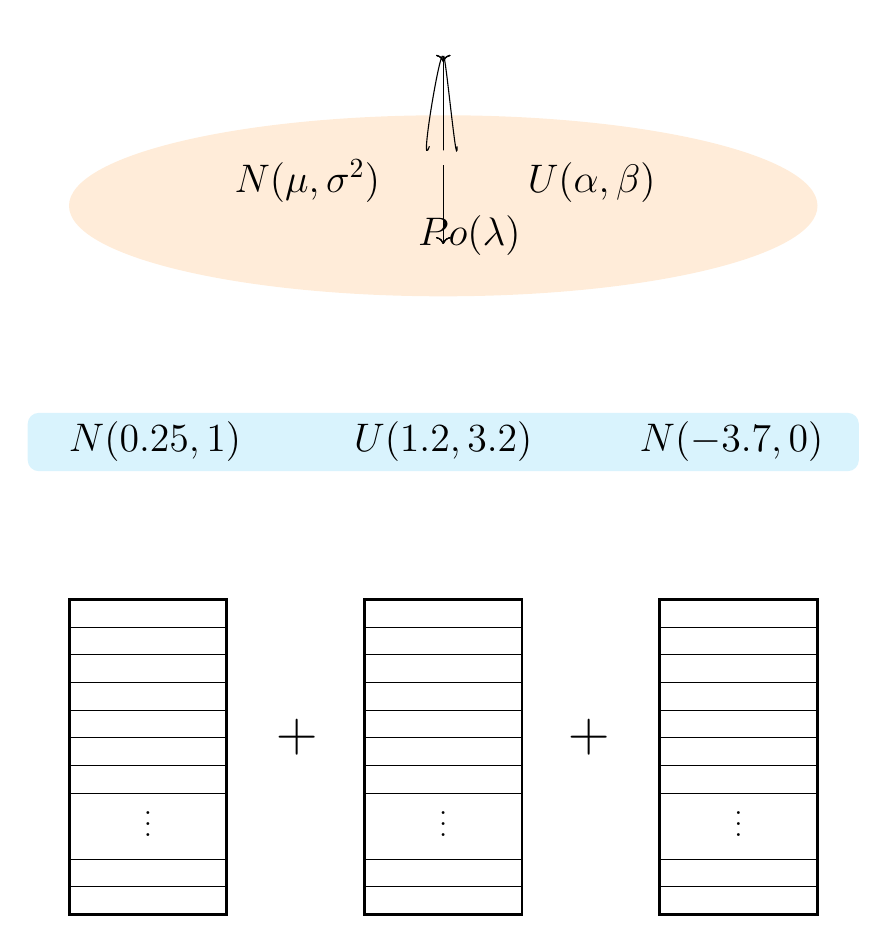
\begin{tikzpicture}

    % Columns
    \path (-2.75, -10) pic {column=7}
          (1, -10) pic {column=7}
          (4.75, -10) pic {column=7};

    \node at (-1.85, -7.75) {\huge \(+\)};
    \node at (1.85, -7.75) {\huge \(+\)};

    % Distribution families
    \node[ellipse, fill=orange!15] (dists) at (0, -1) {\Large%
        \begin{tabular}{c}
            \tikz[baseline, inner sep=0] \node[anchor=base] (normal)
                {\(N(\mu, \sigma^2)\)};
            \qquad
            \tikz[baseline, inner sep=0] \node[anchor=base] (uniform)
                {\(U(\alpha, \beta)\)};
            \\
            {} \quad \(Po(\lambda)\)
        \end{tabular}
    };

    % Metadata
    \node[fill=cyan!15, minimum width=3cm, rounded corners] (metadata) at
        (0, -4) {\Large%
            \tikz[baseline, inner sep=0] \node[anchor=base] (norm1)
                {\(N(0.25, 1)\)};
            \quad
            \tikz[baseline, inner sep=0] \node[anchor=base] (uniform1)
                {\(U(1.2, 3.2)\)};
            \quad
            \tikz[baseline, inner sep=0] \node[anchor=base] (norm2)
                {\(N(-3.7, 0)\)};
        };
 
    % Connecting family to metadata
    \draw[->] ([xshift=-5pt] normal.south)
        to [out=250, in=90] ([yshift=20pt] norm1);

    \draw[->] (uniform) to [out=270, in=90] ([yshift=20pt] uniform1);

    \draw[->] ([xshift=5pt] normal.south)
        to [out=270, in=90] ([yshift=20pt] norm2);

    % Connecting metadata to columns
    \draw[->] ([yshift=-10pt] norm1.south) -- ++(0, -1);
    \draw[->] ([yshift=-10pt] uniform1.south) -- ++(0, -1);
    \draw[->] ([yshift=-10pt] norm2.south) -- ++(0, -1);

\end{tikzpicture}

    }
}

\frame{%
    \resizebox{\textwidth}{!}{%
        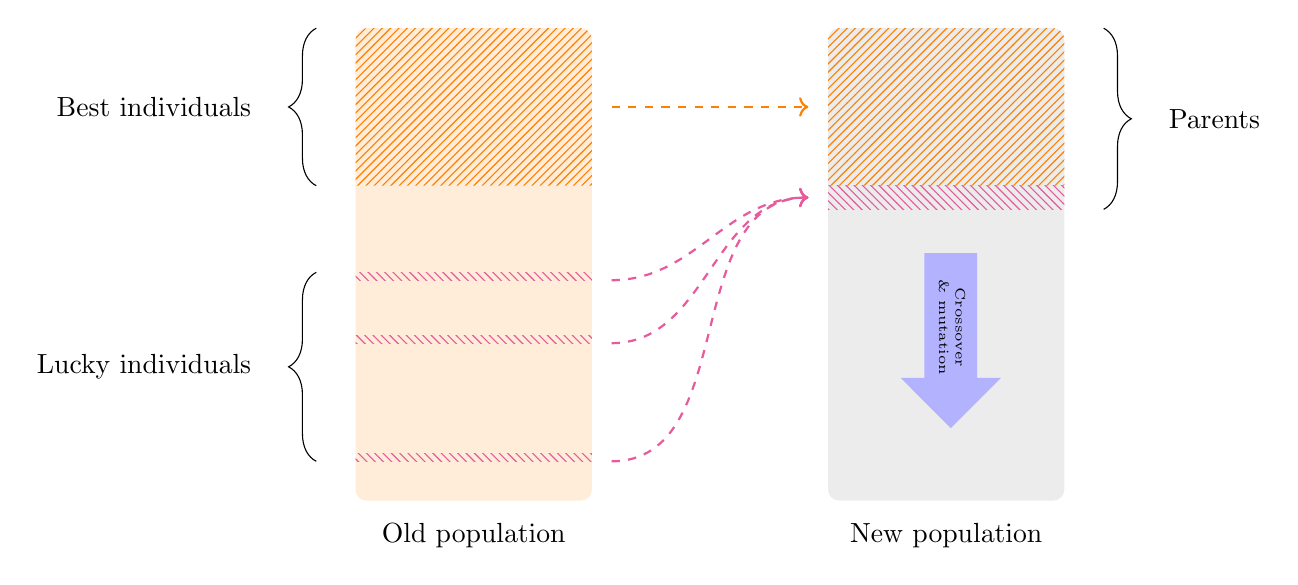
\begin{tikzpicture}

    \fill[orange!15, rounded corners] (0, 0) rectangle (3, -6)
        node[below=90pt, midway] {\color{black} Old population};
    \fill[rounded corners, gray!15] (6, 0) rectangle (9, -6)
        node[below=90pt, midway] {\color{black} New population};

    \fill[pattern=north east lines, pattern color=orange]
        (0, -2) --
        ++(3, 0) {[rounded corners] --
        ++(0, 2) --
        ++(-3, 0)} --
        cycle
        {};
   
    \draw[->, dashed, orange, thick] (3.25, -1) to (5.75, -1);

    \fill[pattern=north east lines, pattern color=orange]
        (6, -2) --
        ++(3, 0) {[rounded corners] --
        ++(0, 2) --
        ++(-3, 0)} --
        cycle
        {};

    \foreach \val in {-5.5, -4, -3.2} {%
        \fill[pattern=north west lines, pattern color=magenta!85]
            (0, \val) rectangle (3, \val+0.1);
        \draw[->, dashed, magenta!85, thick]
            (3.25, \val) to [out=0, in=180] (5.75, -2.15);
    };

    \fill[pattern=north west lines, pattern color=magenta!85]
        (6, -2.3) rectangle (9, -2);

    \draw[decorate, decoration={brace, amplitude=10pt}] (-0.5, -2) -- (-0.5, 0)
        node[midway, left=20pt] {Best individuals};
    \draw[decorate, decoration={brace, amplitude=10pt}] (-0.5, -5.5) -- (-0.5, -3.1)
        node[midway, left=20pt] {Lucky individuals};
    \draw[decorate, decoration={brace, amplitude=10pt}] (9.5, 0) -- (9.5, -2.3)
        node[midway, right=20pt] {Parents};

    \node[%
        fill=blue!30, single arrow, minimum height=18mm, minimum width=4mm,
        single arrow head extend=3mm, anchor=north, rotate=-90
    ] at (7.9, -3.8) {\tiny%
        \begin{tabular}{c}
            Crossover \\
            \& mutation
        \end{tabular}
    };

\end{tikzpicture}

    }
}

\frame{%
    \resizebox{\textwidth}{!}{%
        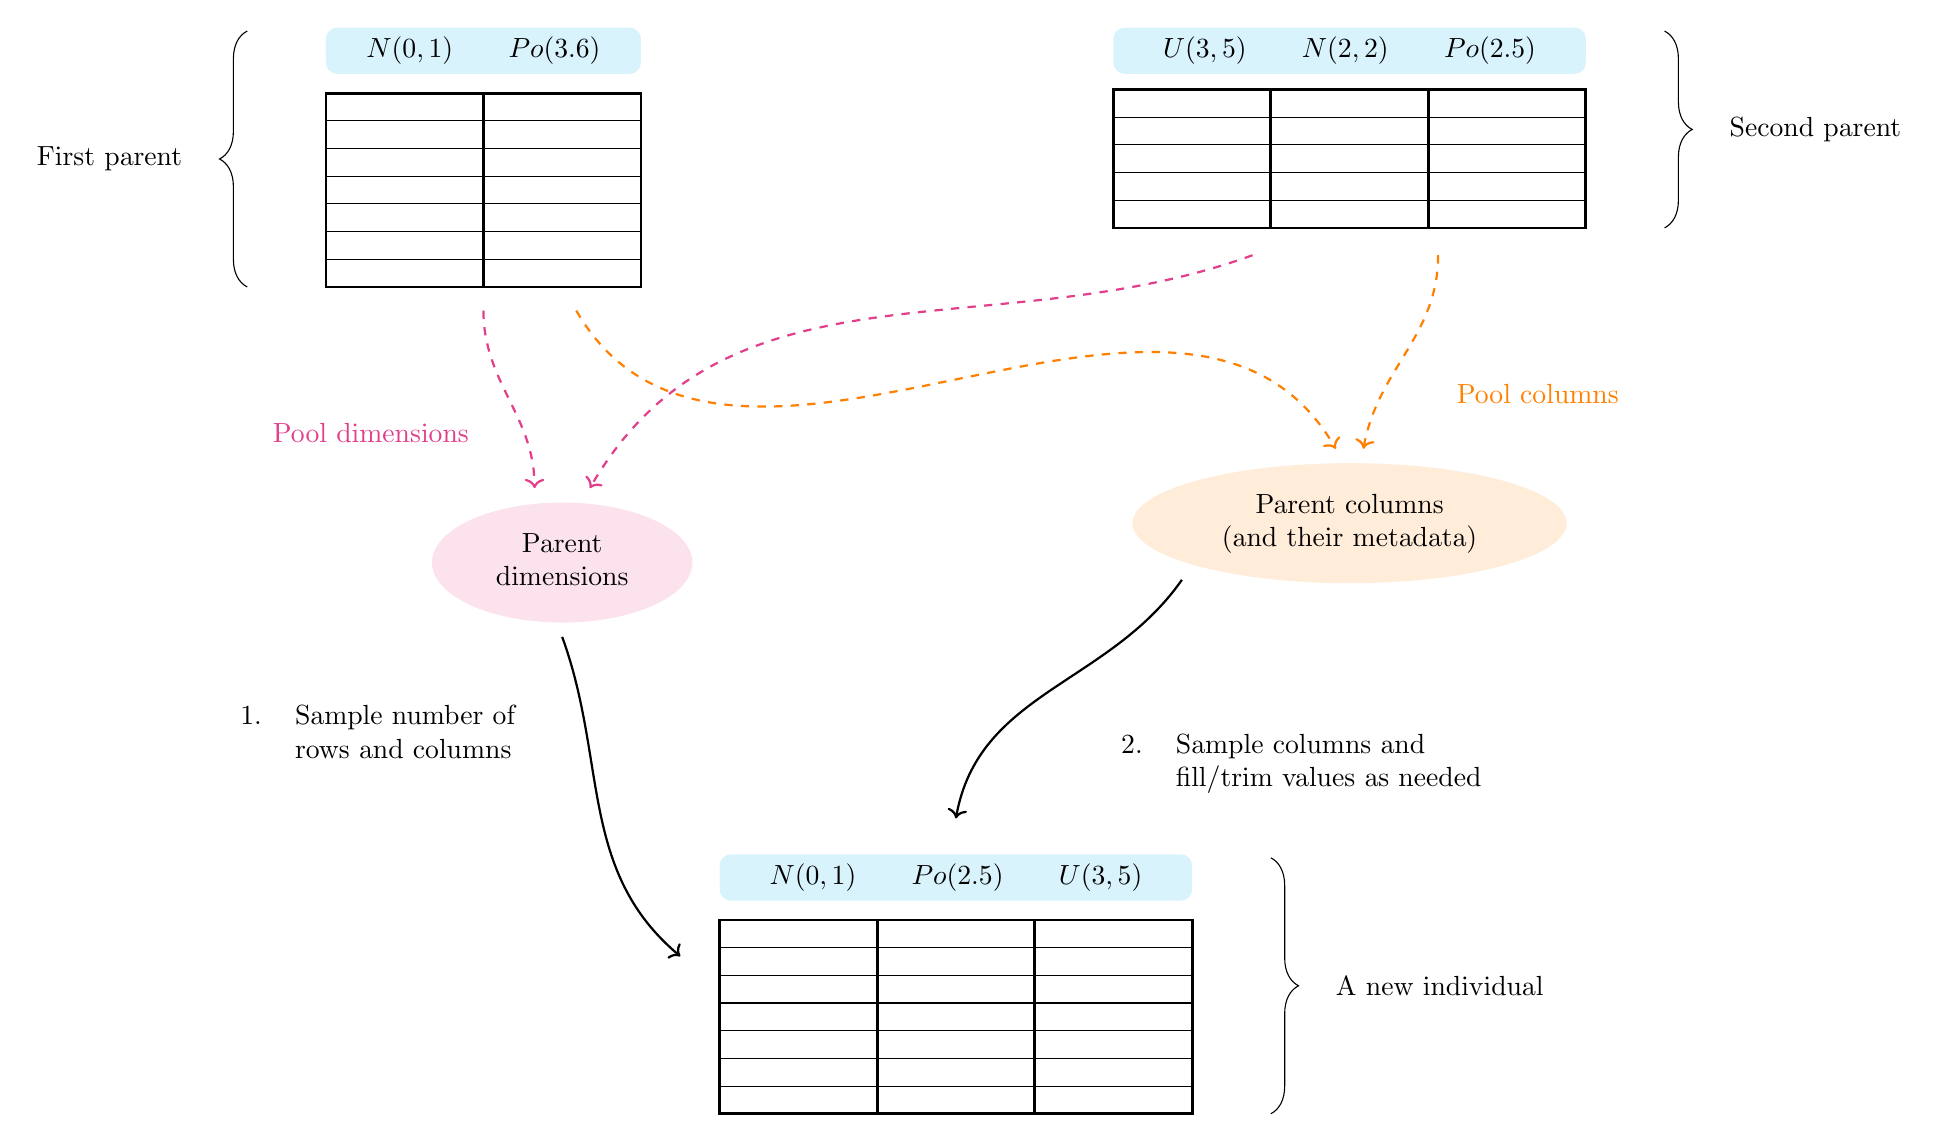
\begin{tikzpicture}

    % First individual
    \path (-2, 1.5) pic {fullcolumn=7}
          (0, 1.5) pic {fullcolumn=7};

    \node (parent1) at (-2, 1.5) {};
    \node[fill=cyan!15, minimum width=4cm, rounded corners] (info1) at (-2, 4.5)
        {\(N(0, 1) \qquad Po(3.6)\)};

    \draw[decorate, decoration={brace, amplitude=10pt}] (-5, 1.5) -- (-5, 4.75)
        node[midway, left=20pt] {First parent};

    % Second individual
    \path (8, 2.25) pic {fullcolumn=5}
          (10, 2.25) pic {fullcolumn=5}
          (12, 2.25) pic {fullcolumn=5};

    \node (parent2) at (10, 1.5) {};
    \node[fill=cyan!15, minimum width=6cm, rounded corners] (info2) at (9, 4.5)
        {\(U(3, 5) \qquad N(2, 2) \qquad Po(2.5)\)};

    \draw[decorate, decoration={brace, amplitude=10pt}] (13, 4.75) -- (13, 2.25)
        node[midway, right=20pt] {Second parent};


    % Pools
    \node[ellipse, fill=magenta!15] (dims) at (-1, -2) {%
        
        \begin{tabular}{c}
            Parent\\
            dimensions
        \end{tabular}
    };

    \node[ellipse, fill=orange!15] (cols) at (9, -1.5) {%
        
        \begin{tabular}{c}
            Parent columns\\
            (and their metadata)
        \end{tabular}
    };


    % Connecting parents to pools
    \draw[->, dashed, orange, thick]%
        ([xshift=30pt, yshift=-5pt] parent1.south east)
        to [out=300, in=120] ([xshift=-5pt, yshift=5pt] cols.north);

    \draw[->, dashed, orange, thick]
        ([yshift=20pt, yshift=-5pt] parent2.south east)
        to [out=270, in=80] ([xshift=5pt, yshift=5pt] cols.north)%
        node[right=30pt, yshift=20pt] {Pool columns};

    \draw[->, dashed, magenta, thick]
        ([xshift=-60pt, yshift=15pt] parent2.south west)
        to [out=200, in=60]
        ([xshift=10pt, yshift=5pt] dims.north);
    \draw[->, dashed, magenta, thick]
        ([yshift=-5pt] parent1.south)
        to [out=270, in=90] ([xshift=-10pt, yshift=5pt] dims.north)
        node[left=20pt, yshift=20pt] {Pool dimensions};


    % The new individual
    \path (3, -9) pic {fullcolumn=7}
          (5, -9) pic {fullcolumn=7}
          (7, -9) pic {fullcolumn=7};

    \node[fill=cyan!15, minimum width=6cm, rounded corners] at (4, -6)
        {\(N(0, 1) \qquad Po(2.5) \qquad U(3, 5)\)};

    \draw[decorate, decoration={brace, amplitude=10pt}] (8, -5.75) -- (8, -9)
        node[midway, right=20pt] {A new individual};


    % Connecting up
    \draw[->, black, thick]
        ([yshift=-5pt] dims.south)
        to [out=290, in=140]
        (0.5, -7)
        node[left=50pt, yshift=80pt] {%
            \begin{tabular}{ll}
                1. & Sample number of\\
                {} & rows and columns
            \end{tabular}
        };

    \draw[->, black, thick]
        ([xshift=-5pt, yshift=-5pt] cols.south west)
        to [out=235, in=80]
        (4, -5.25)
        node[right=50pt, yshift=20pt] {%
            
            \begin{tabular}{ll}
                2. & Sample columns and\\
                {} & fill/trim values as needed
            \end{tabular}
        };

\end{tikzpicture}

    }
}

\frame{%
    \resizebox{\textwidth}{!}{%
        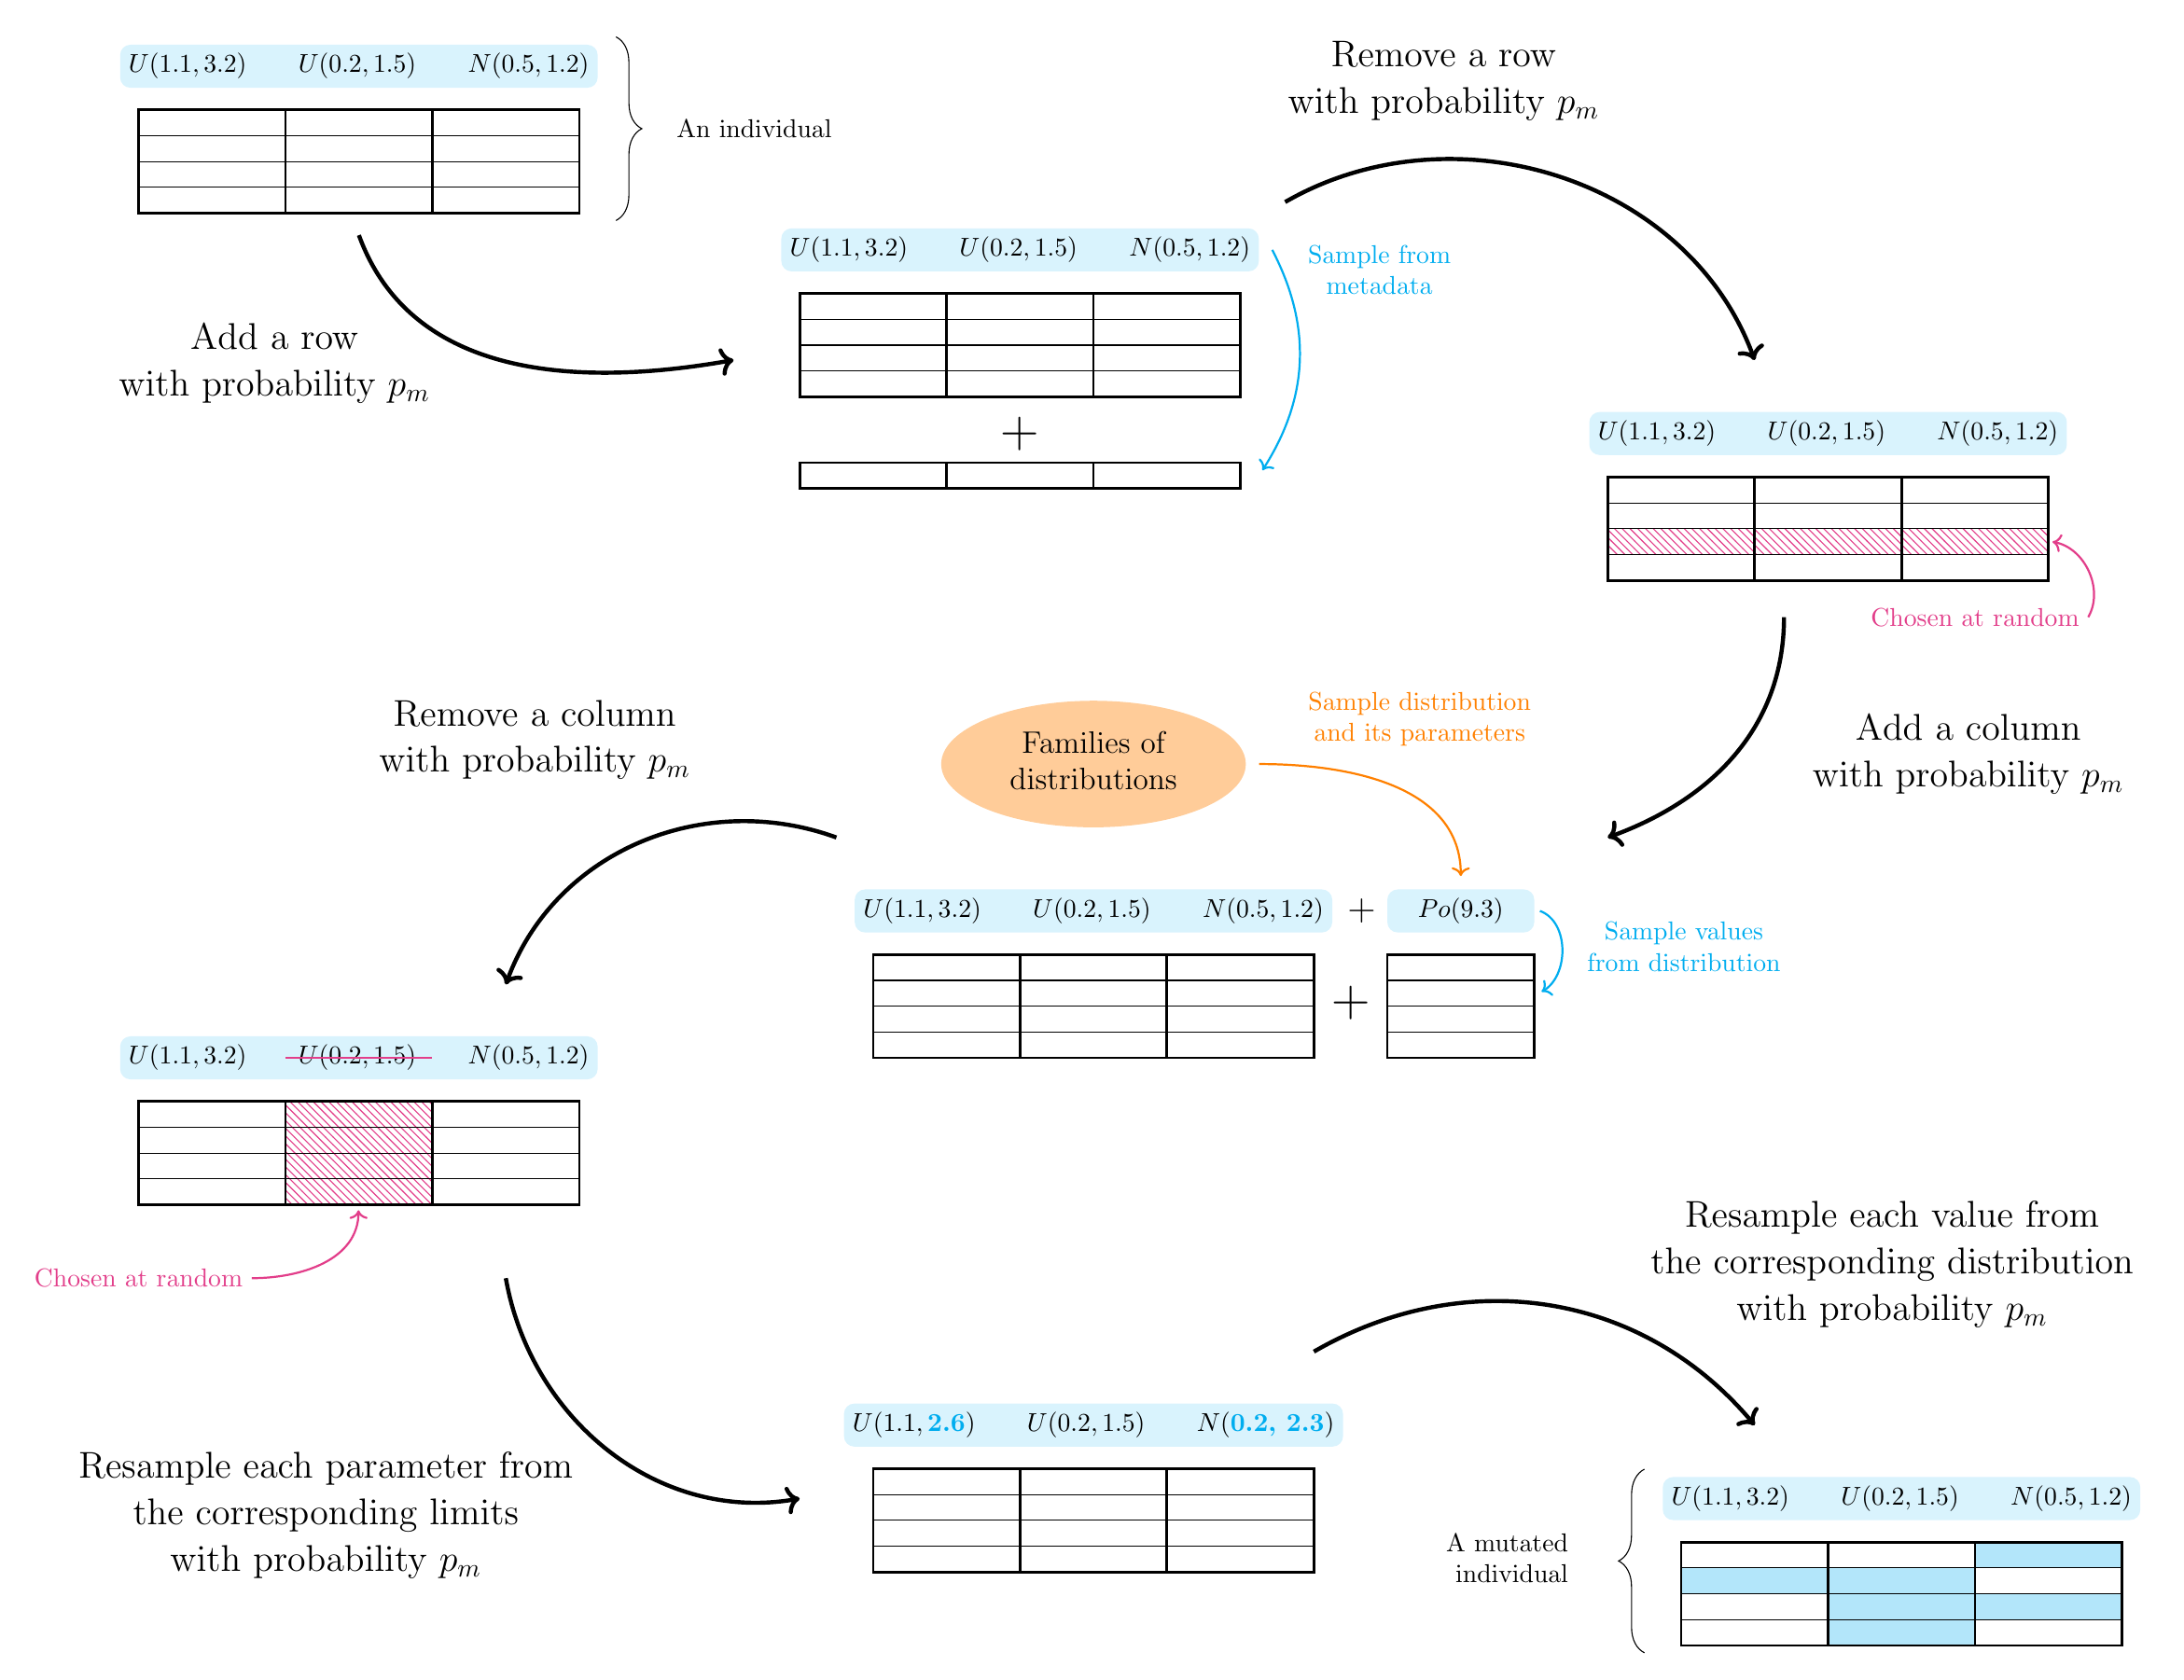
\begin{tikzpicture}

    % Individual
    \path (0, 1.5) pic {fullcolumn=4}
          (2, 1.5) pic {fullcolumn=4}
          (4, 1.5) pic {fullcolumn=4};

    \node (individual) at (1, 1.5) {};
    \node[fill=cyan!15, minimum width=6cm, rounded corners] at (1, 3.5)
        {\(U(1.1, 3.2) \qquad U(0.2, 1.5) \qquad N(0.5, 1.2)\)};

    \draw[decorate, decoration={brace, amplitude=10pt}] (4.5, 3.9) -- (4.5, 1.4)
        node[midway, right=20pt] {An individual};


    % Adding a row
    \draw[->, black, ultra thick]
        ([yshift=-5pt] individual.south)
        to [out=290, in=190]
        node[left=50pt, below, pos=0.2] {\Large%
        \begin{tabular}{c}
            Add a row\\
            with probability \(p_m\)
        \end{tabular}
        } (6.1, -0.5);

    \path (9, -1) pic {fullcolumn=4}
          (11, -1) pic {fullcolumn=4}
          (13, -1) pic {fullcolumn=4};
 
    \node[fill=cyan!15, minimum width=6cm, rounded corners] (r-info) at (10, 1)
        {\(U(1.1, 3.2) \qquad U(0.2, 1.5) \qquad N(0.5, 1.2)\)};

    \path (9, -2.25) pic {fullcolumn=1}
          (11, -2.25) pic {fullcolumn=1}
          (13, -2.25) pic {fullcolumn=1};

    \node (new-row) at (13, -2) {};
    \node (row-plus) at (10, -1.5) {\huge\(+\)};

    \draw[->, cyan, thick]
        ([xshift=5pt] r-info.east)
        to [bend left=30]
        node[right, pos=0.1] {%
            \begin{tabular}{c}
                Sample from\\
                metadata
            \end{tabular}
        } ([xshift=5pt] new-row.east);


    % Deleting a row
    \draw[->, black, ultra thick]
        ([xshift=10pt, yshift=10pt] r-info.north east)
        to [out=30, in=110]
        node[right=20pt, above=10pt, pos=0.2] {\Large%
        \begin{tabular}{c}
            Remove a row\\
            with probability \(p_m\)
        \end{tabular}
        } (20, -0.5);

    \fill[pattern=north west lines, pattern color=magenta]
        (17.99, -3.15) rectangle (24, -2.8)
        node[right=80pt, midway] (row-remove) {};

    \path (20, -3.5) pic {fullcolumn=4}
          (22, -3.5) pic {fullcolumn=4}
          (24, -3.5) pic {fullcolumn=4};

    \node[fill=cyan!15, minimum width=6cm, rounded corners] at (21, -1.5)
    {\(U(1.1, 3.2) \qquad U(0.2, 1.5) \qquad N(0.5, 1.2)\)};

    \node (delete-row) at (23, -4) {\color{magenta} Chosen at random};

    \draw[->, magenta, thick]
        (delete-row.east) to [out=60, in=-10] (row-remove.east);


    % Adding a column
    \draw[->, black, ultra thick]
        (20.4, -4) to [out=270, in=20]
        node[right=20pt, pos=0.5] {\Large%
            \begin{tabular}{c}
                Add a column\\
                with probability \(p_m\)
            \end{tabular}
        } (18, -7);

    \node[ellipse, fill=orange!40] (dists) at (11, -6) {\large%
        \begin{tabular}{c}
            Families of\\
            distributions
        \end{tabular}
    };

    \path (10, -10) pic {fullcolumn=4}
          (12, -10) pic {fullcolumn=4}
          (14, -10) pic {fullcolumn=4};
 
    \node[fill=cyan!15, minimum width=6cm, rounded corners] at (11, -8)
        {\(U(1.1, 3.2) \qquad U(0.2, 1.5) \qquad N(0.5, 1.2)\)};

    \node (info-plus) at (14.65, -8) {\Large\(+\)};
    \node (col-plus) at (14.5, -9.25) {\huge\(+\)};

    \path (17, -10) pic {fullcolumn=4};
    \node[fill=cyan!15, minimum width=2cm, rounded corners] (c-info) at (16, -8)
        {\(Po(9.3)\)};

    \draw[->, orange, thick]
        ([xshift=5pt] dists.east)
        to [out=0, in=90] node[right=10pt, above=10pt, pos=0.5] {%
            \begin{tabular}{c}
                Sample distribution\\
                and its parameters
            \end{tabular}
        } ([yshift=5pt] c-info.north);

    \draw[->, cyan, thick]
        ([xshift=2pt] c-info.east)
        to [out=-20, in=30]
        node[right, pos=0.5] {%
            \begin{tabular}{c}
                Sample values\\
                from distribution
            \end{tabular}
        } (17.1, -9.1);


    % Deleting a column
    \draw[->, black, ultra thick]
        (7.5, -7) to [out=160, in=70]
        node[left=70pt, above=10pt, pos=0.3] {\Large%
            \begin{tabular}{c}
                Remove a column\\
                with probability \(p_m\)
            \end{tabular}
        } (3, -9);

    \fill[pattern=north west lines, pattern color=magenta]
        (-0.01, -12) rectangle (2, -10.6)
        node[below=15pt, midway] (col-remove) {};

    \path (0, -12) pic {fullcolumn=4}
          (2, -12) pic {fullcolumn=4}
          (4, -12) pic {fullcolumn=4};
    \node[fill=cyan!15, minimum width=6cm, rounded corners] at (1, -10)
        {\(U(1.1, 3.2) \qquad U(0.2, 1.5) \qquad N(0.5, 1.2)\)};

    \draw[thick, magenta] (0, -10) -- (2, -10);

    \node (delete-col) at (-2, -13) {\color{magenta} Chosen at random};
    \draw[->, magenta, thick]
        (delete-col.east) to [out=0, in=270] (col-remove.south);


    % Mutate column parameters
    \draw[->, black, ultra thick]
        (3, -13) to [out=280, in=190]
        node[left=80pt, below=30pt, pos=0.2] {\Large%
            \begin{tabular}{c}
                Resample each parameter from\\
                the corresponding limits\\
                with probability \(p_m\)
            \end{tabular}
        } (7, -16);

    \path (10, -17) pic {fullcolumn=4}
          (12, -17) pic {fullcolumn=4}
          (14, -17) pic {fullcolumn=4};

    \node[fill=cyan!15, minimum width=6cm, rounded corners] at (11, -15)
        {\(%
            U(1.1, \textbf{\textcolor{cyan}{2.6}})
            \qquad U(0.2, 1.5) \qquad
            N(\textbf{\textcolor{cyan}{0.2, 2.3}})
        \)};


    % Mutate values
    \draw[->, black, ultra thick]
        (14, -14) to [out=30, in=130]
        node[right=90pt, above, pos=0.75] {\Large%
            \begin{tabular}{c}
                Resample each value from\\
                the corresponding distribution\\
                with probability \(p_m\)
            \end{tabular}
        } (20, -15);


    \fill[cyan!30] (19, -17.3) rectangle (23, -16.95);

    \fill[cyan!30] (21, -18) rectangle (23, -17.3);
    
    \fill[cyan!30] (23, -16.95) rectangle (25, -16.6);
    \fill[cyan!30] (23, -17.65) rectangle (25, -17.3);

    \path (21, -18) pic {fullcolumn=4}
          (23, -18) pic {fullcolumn=4}
          (25, -18) pic {fullcolumn=4};

    \node[fill=cyan!15, minimum width=6cm, rounded corners] at (22, -16)
        {\(U(1.1, 3.2) \qquad U(0.2, 1.5) \qquad N(0.5, 1.2)\)};

    \draw[decorate, decoration={brace, amplitude=10pt}]
        (18.5, -18.1) -- (18.5, -15.6)
        node[midway, left=20pt] {%
            \begin{tabular}{r}
                A mutated\\
                individual
            \end{tabular}
        };


\end{tikzpicture}

    }
}

\frame{%
    \tiny{%
    \begin{itemize}
        \item A fitness function, \(f\), which acts on a single dataset
        \item A population size, \(N \in \mathbb{N}\)
        \item Limits on the number of rows a dataset can have:
            \[
                R \in \left\{%
                    (r_{\min}, r_{\max})
                    \in \mathbb{N}^2~|~r_{\min} \leq r_{\max}
                \right\}
            \]
        \item Limits on the number of columns a dataset can have:
            \[
                C := \left(C_1, \ldots, C_{|\mathcal{P}|}\right)
                ~\text{where}~
                C_j \in \left\{ (c_{\min}, c_{\max}) \in {%
                    \left(\mathbb{N}\cup\{\infty\}\right)
                }^2~|~c_{\min} \leq c_{\max}\right\}
            \]
            for each \(j = 1, \ldots, |\mathcal{P}|\)
        \item A set of probability distribution families, \(\mathcal{P}\). Each
            family in this set has some parameter limits which form a part of
            the overall search space
        \item A probability vector to sample distributions from \(\mathcal{P}\),
            \(w = \left(w_1, \ldots, w_{|\mathcal{P}|}\right)\)
        \item A maximum number of iterations, \(M \in \mathbb{N}\)
        \item Two selection parameters: one to indicate the proportion of the
            fittest individuals to carry forward, \(b \in [0, 1]\), and the
            other to allow for a small proportion of ``lucky'' individuals in
            the next generation, \(l \in [0, 1]\)
        \item A mutation probability, \(p_m \in [0, 1]\)
        \item A shrink factor, \(s \in [0, 1]\). The relative size of a
            component of the search space to be retained after adjustment
    \end{itemize}
    }
}

\section{Some example use cases}

\frame{%
    Given a dataset \(X\), \alert{maximise} \(f\) where:

    \[
        f(X) := \max_{a, b~\in \{(0, 1), (1, 0)\}}%
        \left\{%
            Var \left(X^{(a)}\right) - \max_i \left|X_{i}^{(b)} - 1\right|
        \right\}
    \]
}

\frame{%
    \centering
    \begin{figure}
        \animategraphics[%
            loop,controls,width=\textwidth%
        ]{1}{img/circle/epoch_}{0}{100}
    \end{figure}
}

\frame{%
    \centering
    \begin{figure}
        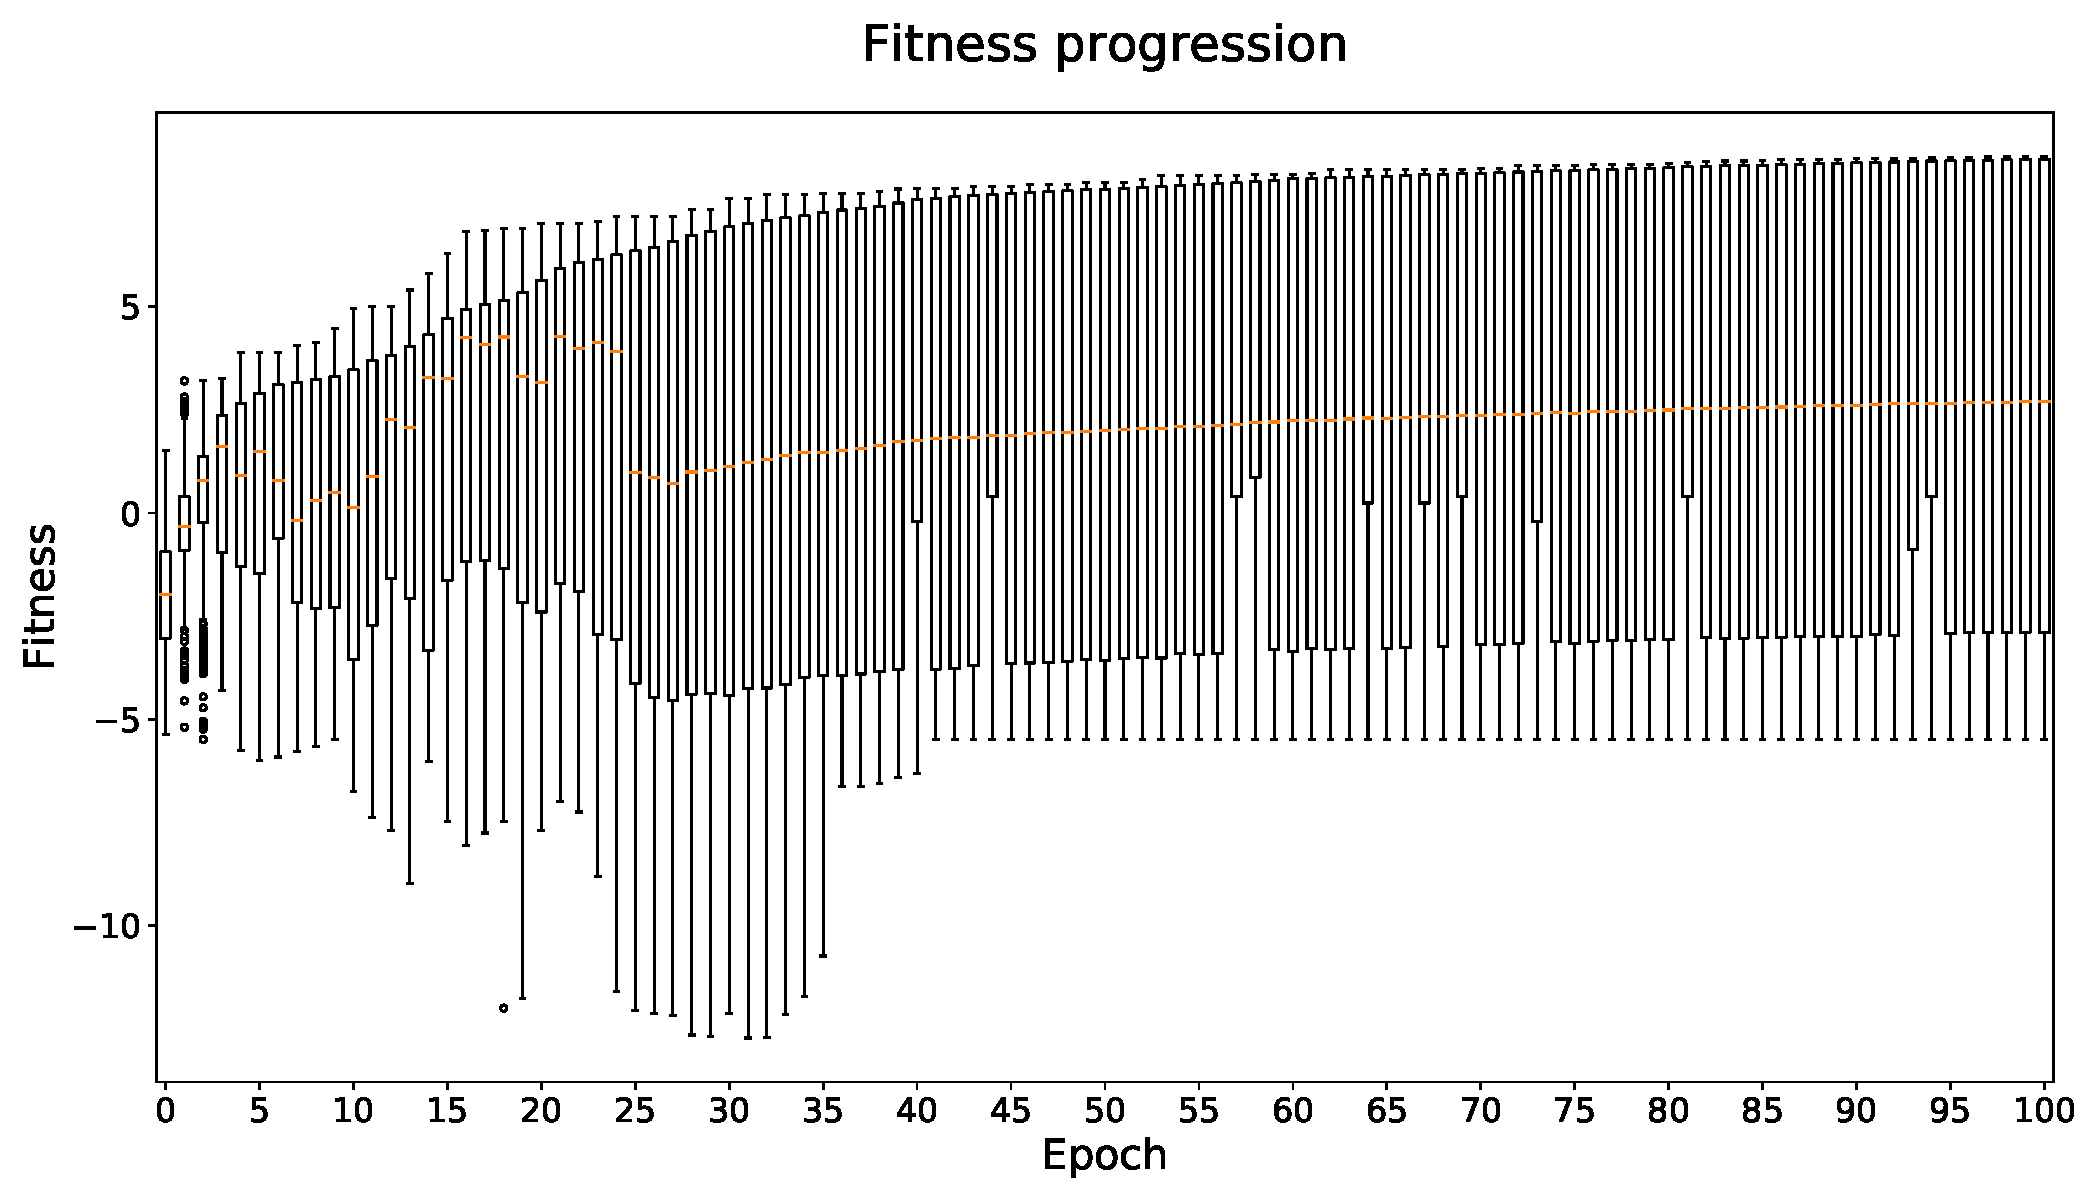
\includegraphics[width=\textwidth]{img/circle/fitness.pdf}
    \end{figure}
}

\frame{%
    \begin{algorithm}[H]
        \KwIn{A dataset (column) \(X\), some sampling fraction \(p\)}
        \KwOut{An estimate for the mean of \(X\)}

        \(Y \gets\) a random sample of \(\left\lfloor p|X| \right\rfloor\)
        entries from \(X\)\;
        evaluate the mean of \(Y\):
        \[
            \bar Y = \frac{1}{|Y|} \sum_{i=1}^{|Y|} Y_i
        \]
    \end{algorithm}

    \[\iff f(X) = \bar Y\]
}

\frame{%
    Anscombe's quartet
}

\frame{%
    \centering
    \Huge{\texttt{\$ pip install edo}}
}

\frame{%
    \begin{center}
        \huge{Any questions?}
    \end{center}

    \begin{center}
        \begin{itemize}
            \item[] Henry Wilde
            \item[] \alert{Twitter:} @daffidwilde
            \item[] \alert{Email:} henrydavidwilde@gmail.com
            \item[] \alert{GitHub repository:} \url{%
                https://github.com/daffidwilde/edo
            }
            \item[] \alert{Documentation:} \url{https://edo.readthedocs.io}
        \end{itemize}
    \end{center}
}

\end{document}
